\documentclass[letterpaper]{article}

\usepackage[utf8]{inputenc}
\usepackage{amsmath}
\usepackage{hyperref}
\usepackage{graphicx}
\usepackage{comment}

\graphicspath{ {./images/} }

\title{A DSL for writing safer string manipulation functions in C}
\author{Michael Flanders}
\date{December 16, 2020}

%You can skip explaining the state of the art (i.e., how the problem is solved today).
%Instead, make sure to include a description of your language. Ideally,
%  you present a language tutorial using your previously selected examples. 
%When explaining your design, refer back to the architecture of DSL
%  implementations, similarly to how we asked you about the FFTW architecture
%  in the reading homework. 
%Please make your design description point to the relevant lines of your implementation.
%  Ideally, your doc will include links to the range of code in your github repo. 
%Please share the repo with the user rbodik. 
%Include the answers to the questions from the last slide.
%Please add the answer to the question "What knowledge or skill would have helped you
%  be more successful with the project."  The answers will help us in further upgrading
%  the course. 

\begin{document}
\maketitle

% Overview of project
% what was proposed initially vs what made it into
% the document
% Overview of the sections

\section{Domain}

% Sample problems from slides
% Easy, medium, hard samples

\section{Language description}

% Overview
% Paradigm, immutability, boundedness
% Language constructs, operators
% Ranges, subranges
% For loops

\section{Design and decisions}

\begin{figure}[h]
  \centering
  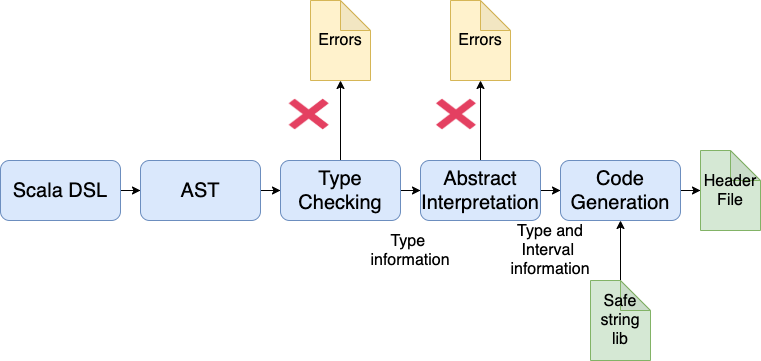
\includegraphics[width=\textwidth]{architecture.png}
  \caption{Diagram of the compiler pipeline}
  \label{fig:pipeline}
\end{figure}

% Overview
% Lexer/parser vs fluent-syntax/call-chaining
% Typechecker
% Abstract interpreter
%  abstract domain
%  vs symbolic execution
% Code generation
%  the safe string library
%  problems (memory leaks)

\section{Discussion}

% Answer the questions from the last slide (of the template?)
% "What knowledge or skill would have helped you be more
%   successful in the project?"

\end{document}
